%Kontext: Admin Dokumentation zum Projekt CodeRed 
%Changelog:
%Timestamp                      Name                      Äderungen und Begründung
%

%Dokumentklasse und einige globale Einstellungen
\documentclass[11pt,a4paper,titlepage,openright,multicol]{scrbook}

%Untersttzung für Zeichen außrhalb des ASCII-Zeichensatzes
\usepackage[utf8]{inputenc}
\usepackage{fontenc}

%Trennungsregeln
\usepackage[ngermanb]{babel}

\usepackage{multicol}

%zahlreiche Pakete und weitere Einstellungen
\usepackage{color}
\usepackage{fancyhdr}

%\usepackage[a4paper,left=3cm,right=1.5cm,headheight=1.5cm]{geometry}
\usepackage{ngerman}
\usepackage[pdftex]{graphicx}

\usepackage[pdftex, bookmarks,
		colorlinks=true,
		linkcolor=black,
		urlcolor=black,
		pdftitle={CodeRed Unterweisung},
		pdfauthor={Marco Benecke, Jan Neuser},
		pdfsubject={Eine Unterweisung in die Software CodeRed}
		pdfkeywords={ADA, Unterweisung, Codered, STSWeilburg}]{hyperref}


\usepackage{longtable}

%Erstellung einer Indexdatei
\usepackage{makeidx}

\usepackage{textcomp}
\usepackage{verbatim}

%Verwendung von Font Type 1 fr bessere Lesbarkeit im Acrobat Reader
\usepackage{pslatex}

%Gliederungstiefe, Makropaket und Einstellung fr das Inhaltsverzeichnis
\usepackage{minitoc}
\setcounter{secnumdepth}{3}
\setcounter{tocdepth}{2}

%Aufnahme der Verzeichnisse (Stichwortverzeichnis, Abbildungs- und Tabellenverzeichnis) ins Inhaltsverzeichnis
\usepackage{tocbibind}

\usepackage{nomencl}

\usepackage{listings}
%in der aktuellen Version des Styles fr listings haben sich einige �derungen ergeben, insbesondere wird label durch number ersetzt, das Stylefile wird nicht mehr ausgeliefert
%\lstset{captionpos=b, frame=trbl, frameround=ffff, labelstyle=\tiny, labelstep=5, firstlabel=1, labelsep=5pt}
%\lstset{captionpos=b, frame=trbl, frameround=ffff, numberstyle=\tiny, stepnumber=5, firstnumber=1, numbersep=5pt, aboveskip=10pt, belowskip=10pt}

% weitere Eigenschaften fr den Abstand des Listings
% aboveskip=10pt, belowskip=10pt

\usepackage{path}

% Das Paket parskip verhindert den Einzug am Anfang neuer Abs�ze und setzt einen sinnvollen Zeilenabstand zwischen den Abs�zen, wirkt sich darber hinaus auch Einrckungen in Aufz�lungen, Listen usw. aus.
\usepackage{parskip}

%sollte Fussnoten in Tabellen erm�lichen, berfordert aber Latex
%\usepackage{./texstyles/ftn}
%\ftn{tabular}

\makeatletter
%Breite fr die Seitennummerierung in Inhaltsverzeichnis
%Vermeidung des Fehlers Overfull \hbox
\renewcommand{\@pnumwidth}{2.5em}

%Abstand zwischen der Abschnittsnummer und der Kapitelberschrift im Inhaltsverzeichnis
\renewcommand*\l@section{\@dottedtocline{1}{1.0em}{2.3em}}
\renewcommand*\l@subsection{\@dottedtocline{2}{3.3em}{3.2em}}
\renewcommand*\l@subsubsection{\@dottedtocline{3}{6.5em}{4.1em}}
\renewcommand*\l@paragraph{\@dottedtocline{4}{9.5em}{5.0em}}
\renewcommand*\l@subparagraph{\@dottedtocline{5}{11.5em}{6.0em}}

%Kapitelnummerierung am Anfang jedes Buches, eingeleitet durch \part zurcksetzen
%Kompiliert jetzt zwar korrekt, verhindert aber ein vernnftiges Bookmarking durch das Paket hyperref
\@addtoreset{chapter}{part}
\makeatother

%Seitennummerierung in arabischen Ziffern
\pagenumbering{arabic}

\makeindex
\makeglossary

%Anfang des Dokuments
\begin{document}

%Einleitung mit eigenen Seitennummerierung
\frontmatter

%Hauptteil
\mainmatter

%Titelseite
%Kontext: Komplettes Handbuch für Codered
%Changelog:
%Timestamp			Name			Äderungen und Begründung
%

\begin{titlepage}

\title{- \textbf{CodeRed} -\\ 
\mbox{Das \textit{Trouble Ticket System}} \\
- der Staatliche Techniker Schule Weilburg  -\\
Administrations Dokumentation}
\author{Marco Benecke \and Jan Neuser}
\date{Ausgabe 0.1 vom \today}

\publishers{Staatliche Techniker Schule Weilburg}

\uppertitleback{

\textbf{Version:} \\
\textbf{Version:} \\
- Projekt Dokumentation\\
- \underline{CodeRed Server Administratio}n \\
- CodeRed Benutzer Dokumentaion \\
% use packages: array
\begin{tabular}{ll}
Thema: & CodeRed - Handbuch - Administration\\
Server & Version: Debian 2.6.12 - Apache2 CTL \\
Datum: &  29.03.06\\ 
Puplic Version: & CodeRed System RC2 \\  
\\
\end{tabular}

\vspace{2cm}

\textbf{Autoren:} \\
Benecke, Marco erreichbar unter \textit{benecke@gmail.com} \\
Neuser, Jan mit \textit{jan@truematrix.de} \\

\vspace{1cm}

\textbf{Korrekturleser:} \\
 Cristine Holzhäuser \\
 Beate Neuser \\
 Anne Neuser \\
}

\lowertitleback{Dieses Buch unterliegt den Grundgedanken der GPL und wird ausschließich mit Hilfe des Satzsystems {\LaTeX} unter Linux geschrieben. Die Veröffentlichung erfolgt als plattformunabhägiges PDF. Vielen Dank.}

\maketitle

\end{titlepage}



%Inhaltsverzeichnis
\tableofcontents

\part{Einleitung}
\label{part:Einleitung}
\chapter{Die Idee}  % Kapitel % Steht dann über dem Text
\label{chapter:Die Idee}  % Steht als Text im Inhaltsverzeichnis
\index{Die Idee} % für das Stichwortverzeichnis

Die Staatliche Technikerschule Weilburg (STSW)
übernimmt seit Jahren verschiedene IT Projekte
von Firmen und Schulen im Rahmen der praktischen
Abschlussprüfungen der angehenden Techniker. \\
\\
Nun stellte sich heraus, dass mit der Zeit
Wartungsarbeiten an den Projekten anfallen oder
dass Defekte behoben werden müssen.
Die Schulen, die selbst keine Ressourcen für die
Problembehebung bündeln konnten, haben sich
wieder an die STSW gewannt, um Hilfe bei ihren
Problemen zu bekommen. \\
\\
Diese Probleme wurden an einen Lehrer weitergeleitet,
dieser löste diese entweder selbst oder
beauftragte einige Studierende mit der Lösung.
Schwierigkeiten bestanden darin, dass meist nur noch die
Dokumentation des Projektes zur Lösungshilfe bereit
steht. Alle Änderungen und evtl. schon vorhandene
gelöste Probleme sind nicht dokumentiert gewesen und gingen
somit immer mit dem Abschluss der Studierenden verloren.\\
\\
Die Lösung für diese vielen Probleme wurde unter dem Namen \textbf{CodeRed} 
entwickelt. Ca ein Jahr hat sich das Team gedanken über eine Lösung und 
deren umsetzung gedanken gemacht. CodeRed verwaltet zentral alle Probleme 
die bei den Klienten entstehen. Das System ist webbasierend und dadurch von jedem 
Anwender mit einem Internetzugang anwendbar. Serviceteams, Clienten, Kontakte oder auch Mentoren können über die Datenbankapplication schnell und einfach ihre Probleme oder Lösungen dokumentieren. \\
\\
Bei der Entwicklung wurde besonders darauf geachtet, die komplexen Abläufe die Auftreten können, klar und einfach zu halten. Niemand sollte eine gößere Einführung in die Software benötigen um sie Nutzen zu können. Deswegen wurde auf neue Technologien die unter dem Begriff Web2.0 in den Fachmedien bekannt geworden sind, großen Wert gelegt.\\
\\
Wir die Entwickler hoffen eine leistungfähige Lösung entwickelt zu haben, die von jedermann bedient werden kann.   

\chapter{Danksagung}  % Kapitel % Steht dann über dem Text
\label{chapter:Danksagung}  % Steht als Text im Inhaltsverzeichnis
\index{Danksagung} % für das Stichwortverzeichnis

Das Projekt CodeRed konnte nur durch die Unterstützung von vielen verschieden Personen und Freien Internet Diensten verwirklicht werden. So möchten wir uns bei allen Menschen und Institutionen für ihre Ideen, Kretik und ihr Lob bedanken. \\
Ein paar Vorbilder und Hilfen für die Umsetzung dieses Projektes waren: 
\\
\textbf{Dienste und Pattformen}
\begin{itemize}
\item \href{http://www.berlios.de}{BerliOS}, die jedem Entwickeler eine sehr gute freie Kommunikatiosplattform zur verfügung stellt,
\item \href{http://www.google.de}{Google}, mit ihren Entwicklungen wie Gmail waren sie ein sehr großes Vorbild in Sachen Anwenderfreundlichkeit. 
\item \href{http://rubyonrails.de}{ROR Entwickler Deutschland}, mit ihrer Hilfe über die Mailingliste haben sie uns über einige Fehler hinweggeholfen
\end{itemize}
\chapter{Entwickler}  % Kapitel % Steht dann über dem Text
\label{chapter:Entwickler}  % Steht als Text im Inhaltsverzeichnis
\index{Entwickler} % für das Stichwortverzeichnis

Als Entwickeler von CoderRed möchten wir uns gerne hier kurz vorstellen, wir stehen allen die weitere Fragen zu diesem Projekt haben natürlich gerne zur Verfügung. \\
\\
Allgemein besteht das Entwickelerteam von CodeRed aus zwei Studierenden der Staatlichen Techniker Schule Weilburg. Wir haben im Jahr 2004 die Ausbildung zum Staatlichen Techniker der Informationstechnik, Schwerpunkt Computersystem und Netzwerktechnik begonnen und Sommer 2005 dieses Projekt übernommen. Für uns stand bei der Übernahme der Aufgabe vorallem eines im Vordergrung, wir wollen unbedingt etwas machen was wir noch nicht beherschen und wir viel Lernen könnten. So war die Entwicklung eines Webbasierenden Trouble Ticket System eine nahe zu ideale Aufgabe, auch wenn wir erst nicht wussten wie wir diese Aufgabe lösen sollten.   
\\
\\
Backend Entwickeler \\
\textbf{Marco Benecke}
\\
\begin{picture}(150,200)

\includegraphics{../bilder/marcob.jpg}
\end{picture}
\\
Marco Benecke \\
Bitzengarten 16 \\
35614 Asslar-Oberlemp \\
\\
\textbf{Konatkt} \\
\begin{itemize}
\item Mobil: 0175 - 74 10 565
\item E-Mail: benecke@gmail.com
\item JabberID: Risktaker@jabber.org 
\item Homepage: \href{http://www.bytes-delivery.de}{bytes-delivery.de}
\end{itemize}
\textbf{Werdegang} \\
\begin{itemize}
\item Realschulabschluss auf der Gesamtschule Asslar-Hermannstein
\item Ausbildung zum Energieelektroniker-Betriebstechnik bei der Buderus Guss GmbH in Wetzlar
\item 5./Technische Schule der Luftwaffe in Erndtebrück Staabsgebiet 6 – Netzbetreuer und Administrator
\item Weiterbildung zum Staatlich geprüften Techniker in Weilburg, Schwerpunkt: Computersystem und Netzwerktechnik	
\end{itemize}
FrontEnd Entwickeler \\
\textbf{Jan Neuser}
\\
\begin{picture}(150,200)

\includegraphics{../bilder/marcob.jpg}
\end{picture}
\\
Jan Neuser \\
Münchbornstr.4 \\
35753 Greifenstein Arborn \\
\\
\textbf{Konatkt} \\
\begin{itemize}
\item Mobil: 0177 - 60 39 783
\item E-Mail: jan@truematrix.de
\item JabberID: nean77@gmail.com 
\item Homepage: \href{http://www.truematrix.de}{truematrix.de}
\end{itemize}
\textbf{Werdegang} \\
\begin{itemize}
\item Realschulabschluss auf der Gesamtschule Driedorf
\item Ausbildung zum IT- Systemelektroniker in Sinn bei der Firma Dietermann \and Heuser GmbH  (Heute: Hees Bürowelt)
\item Stabskompanie Panzerbrigade 14, Stabsdienst - Truppenverwaltung
\item Weiterbildung zum Staatlich geprüften Techniker in Weilburg, Schwerpunkt: Computersystem und Netzwerktechnik	
\end{itemize}




\part{Vorbereitungen}
\label{part:Vorbereitungen}
\input{Zweck}
\chapter{Voraussetzungen }  % Kapitel % Steht dann über dem Text
\label{chapter:Vorausetzungen}  % Steht als Text im Inhaltsverzeichnis
\index{Voraussetzungen} % für das Stichwortverzeichnis

Für eine erfolgreiche Installation eines Servers müssen verschiedene Hardware und Software Vorrausetzungen erfüllt werden. Die folgen Auflistungen beinhalten nur die Groben Hardware Bedingungen und die Hauptsoftware Pakete. Bei der späteren Installationsanleitungen werden noch verschiedene kleiner Pakete installiert, um einen Reibungslosen Betrieb zu gewährleisten. \\
\section{Hardware Vorrausetzungen}
\label{section:Hardware Vorraussetzungen}
\index{Hardware}
\index{Hardware}
\begin{itemize}
\item Intel x86-basierend System 
\item Schnittstellen: 1x LAN
\item Arbeitsspeicher: min 256 MB \footnotemark[1]
\item Laufwerke: 1x DVD Laufwerk
\item HDD: Je nach bedarf! (Aktuell 40 Gb)
\end{itemize}
\footnote[1]{Die Anforderungen an den Arbeitsspeicher steigen schnell, da gerade Datenbank Anwendungen viel Arbeitsspeicher benötigen.}

\section{Software Vorrausetzungen}
\label{section:Software Vorraussetzungen}
\index{Software}
\index{Software}
\begin{itemize}
\item Linux Distribution DVD Debian ab Version 3.1 - \href{http://www.Debian.org}{http://www.Debian.org}
\item Apache 2 Webserver mit Fast CGI -
\href{http://www.apache2.org}{http://www.apache2.org}
\item MySQL Server ab Version 4 - 
\href{http://dev.mysql.com}{http://www.mysql.com}
\item Ruby Installations Paket mit Gems Paketverwaltung - \href{http://www.ruby-lang.org/en/}{http://www.ruby-lang.org/en}
\item Ruby on Rails Framework -
\href{http://www.rubyonrails.com/}{http://www.rubyonrails.com}
\end{itemize}

\chapter{Zeitplan}  % Kapitel % Steht dann über dem Text
\label{chapter:Zeitplan}  % Steht als Text im Inhaltsverzeichnis
\index{Zeitplan} % für das Stichwortverzeichnis
\begin{figure}[h]
\begin{center}
   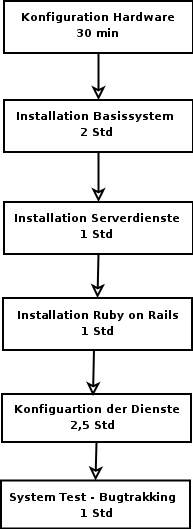
\includegraphics[width=5cm]{../bilder/Zeitplaninstall.png}
   \caption{Zeitplan Systeminstallation}
   \label{Zeitplan-Ablauf}
\end{center}
\end{figure}

Die Grafik zeigt den ideal Ablauf einer Serverinstallation für einen CodeRed Server. Probleme mit der Hardware oder auch mit der Anbindung sind hier nicht berücksichtigt. Die Intallation kann sich bei Problemen, die nichts direkt mit dem eigentlichen System zutun haben, um eine nicht bestimmbare Zeit verlängern.




\part{Der Server}
\label{part:Der Server}
\chapter{Basis Installation}  % Kapitel % Steht dann über dem Text
\label{Basis Installation}  % Steht als Text im Inhaltsverzeichnis
\index{Basis Installation} % für das Stichwortverzeichnis

Vorstellung unsers Ausgangsserver
Hardware , Photo 

\section{BIOS Einstellungen}
\label{section:BIOS Einstellungen}
\index{BIOS Einstellungen}
\index{BIOS Einstellungen}
Im BIOS des Systems wurden folgende Anpassungen gemacht:
\begin{itemize}
\item No halt on any error
\item acpi/apm ausgeschaltet
\item boot reihenfolge auf cd/hd/nw/fd
\item Biospass nicht gesetzt
\end{itemize}
Hauptsächlich wurde dafür gesorgt das der Server auch ohne den Anschluss einer Tastatur starten wird. Zudem wurden alle Power Save Modis abgeschaltet um die Zugrifzeiten auf Datenbestände nicht unnötig zu verlangsamen.
 
\section{Debian Grundsystem}
\label{section:Debian Grundsystem}
\index{Basis Installation Debian}
\index{Debian Grundsystem}
Installation des Debianbasissystems von einer DVD \\
\\
\textbf{1) Einlegen der Debian CD --boot parameter \glqq linux26\grqq} \\
Der Debian Server soll mit dem Kernel 2.6.x laufen, deswegen wird als Startoption $>$ linux26 übergeben. \\
\\
\textbf{2) Basisinstallation}
\begin{table}[htbp]
\begin{center}
\begin{tabular*}{0.95\textwidth}{p{0.3\textwidth}p{0.6\textwidth}}
\hline
\textbf{Frage?} & \textbf{Auswahl} \\
\hline
Sprachenauswahl: & Deutsch \\
Landgebiet: & Deutschland \\
Tastatulayout: & Deutsch \\
Rechnername: & codered \\
\hline
\end{tabular*}
\caption{Grundeinstellungen System}
\label{table:Grundeinstellungen System}
\end{center}
\end{table}
\begin{table}[htbp]
\begin{center}
\begin{tabular*}{0.95\textwidth}{p{0.3\textwidth}p{0.6\textwidth}}
\hline
\textbf{Frage?} & \textbf{Auswahl} \\
\hline
ip-address & 192.168.42.42 \\
subnetmask & 255.255.255.0 \\
gateway & 192.168.42.1 \\
DNS & (erstmal) 4.2.2.2 \\
\hline
\end{tabular*}
\caption{Netzwerk Einstellungen}
\label{table:Netzwerk Einstellungen}
\end{center}
\end{table}
\begin{table}[htbp]
\begin{center}
\begin{tabular*}{0.95\textwidth}{p{0.1\textwidth}p{0.2\textwidth}p{0.1\textwidth}p{0.4\textwidth}}
\hline
\textbf{Partition} & \textbf{Mount Point} & \textbf{Größe} & \textbf{Reserve} \\
\hline
hda1 & boot & 200mb & keine reserve für root \\
hda5 & / & 5gb & 10\%  reserve für root \\
hda6 & /var & 30gb & 15\%  reserve für root \\
hda7 & /tmp & 2.8gb & 10\%  reserve für root \\
hda8 & swap & 2gb & keine reserve für root \\
\hline
\end{tabular*}
\caption{Festplatten Nutzung}
\label{table:Festplatten Nutzung}
\end{center}
\end{table}


\section{Debian Grundkonfiguration}
\label{section:Debian Grundkonfiguration}
\index{Konfiguration des Grunssystems}
\index{Debian Grundkonfiguration}

\begin{itemize}
\item \glqq NEIN\grqq --Hardware Uhr steht nicht auf gmt
\item \glqq JA\grqq -- Zeitzone ist Berlin
\item Rootpasswort \textbf{mzkeWgDCaJyhaPCD7PQ}
\item Es werden keine weiteren Benutzer am System angelegt \textit{(abrechen)}
\item apt-setup   --Die CDs eingelesen lassen
\item Sprachbezogene Einstellungen bestätigen
\item \glqq MTA\grqq  --Keine Konfiguration vorgenommen 
\end{itemize}

\input{pro_system} 

\part{Ruby on Rails}
\label{part:Ruby on Rails}
%\input{Installation_ruby}
%\input{Konfiguration_ruby}

\part{Dienste}
\label{part:Dienste}
%\input{Dienste}

\part{Future List}
\label{part:Future List}
%\input{future}

\part{Kopiervorlagen}
\label{part:Kopiervorlagen}

%Anhang
\backmatter
\appendix
\part{Anhang}
\label{part:Anhang}

%Entwurf von Tobias Mucke
%Erg�zungen von Michael Petter
%Kontext: SuSE 8.0
%Changelog:
%Timestamp                       Name                       �derungen und Begrndung
%26. Oktober 2002           Tobias Mucke        erweitert und korrigiert

\chapter{Literaturverzeichnis}
\begin{description}
\item{[1]}
Marco Benecke: \textit{Linux Installation, Konfiguration, Anwendung},
noch in planung :)

\end{description}






\printglossary

%Abbbildungsverzeichnis
\listoffigures

%Tabellenverzeichnis
\listoftables

%Listingverzeichnis
\lstlistoflistings

% Stichwortverzeichnis
\printindex

%Ende des Dokuments
\end{document}
